% #######################################
% ########### FILL THESE IN #############
% #######################################
\def\mytitle{MATLAB Graphic Equaliser -- Report}
\def\mykeywords{Fill, These, In, So, google, can, find, your, report}
\def\myauthor{Miles Budden C1769331}
\def\contact{BuddenM@Cardiff.ac.uk}
\def\mymodule{Scientific Computing (CM2208)}
% #######################################
% #### YOU DON'T NEED TO TOUCH BELOW ####
% #######################################
\documentclass[10pt, a4paper]{article}
\usepackage[a4paper,outer=1.5cm,inner=1.5cm,top=1.75cm,bottom=1.5cm]{geometry}
\twocolumn
\usepackage{graphicx}
\graphicspath{{./images/}}
%colour our links, remove weird boxes
\usepackage[hyphens]{url}
\usepackage[hidelinks]{hyperref}
%Stop indentation on new paragraphs
\usepackage[parfill]{parskip}
\usepackage{amssymb}
\usepackage{amsmath}
\usepackage{pgfplots}




%Cardiff logo top right
\usepackage{watermark}
%Lorem Ipusm dolor please don't leave any in you final report ;)
\usepackage{lipsum}
\usepackage{xcolor}
\usepackage{listings}
\usepackage{minted}
\setminted{
    frame=lines,
    framesep=2mm,
    baselinestretch=1.2,
    fontsize=\footnotesize,
    breaklines
}
%give us the Capital H that we all know and love
\usepackage{float}
%tone down the line spacing after section titles
\usepackage{titlesec}
%Cool maths printing
\usepackage{amsmath}
%PseudoCode
\usepackage{algorithm2e}
\usepackage{natbib}

\titlespacing{\subsection}{0pt}{\parskip}{-3pt}
\titlespacing{\subsubsection}{0pt}{\parskip}{-\parskip}
\titlespacing{\paragraph}{0pt}{\parskip}{\parskip}
\newcommand{\figuremacro}[5]{
    \begin{figure}[#1]
        \centering
        \includegraphics[width=#5\columnwidth]{#2}
        \caption[#3]{\textbf{#3}#4}
        \label{fig:#2}
    \end{figure}
}


% \thiswatermark{\centering \put(400.5,-100.0){
\includegraphics[scale=0.2]{logo}} }
\title{\mytitle}
\author{\myauthor\hspace{1em}\\\contact\\Cardiff University\hspace{0.5em}-\hspace{0.5em}\mymodule}
\date{}
\hypersetup{pdfauthor=\myauthor,pdftitle=\mytitle,pdfkeywords=\mykeywords}
\sloppy
% #######################################
% ########### START FROM HERE ###########
% #######################################
\begin{document}
\maketitle
\tableofcontents
\section{Design}
\begin{figure}[h]
    \centering
    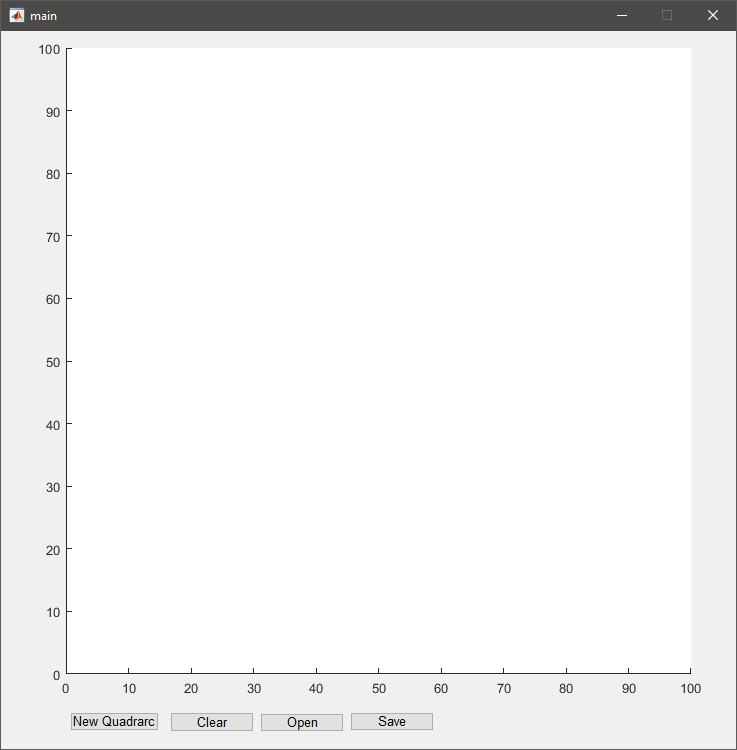
\includegraphics[width=0.25\textwidth]{empty}
    \caption{A blank plot}
    \label{fig:empty}
\end{figure}
\section{Implementation}
\section{Algorithmic Overview}




















% \section{Operation}
% \subsection{Plotting Quadrarcs}
% The tool can be started by loading the \texttt{main.fig} file. This file relies on \texttt{main.m} for functionality. When run, the user is presented with a axis as can be seen in Figure \ref{fig:empty}. 

% \begin{figure}[h]
%     \centering
%     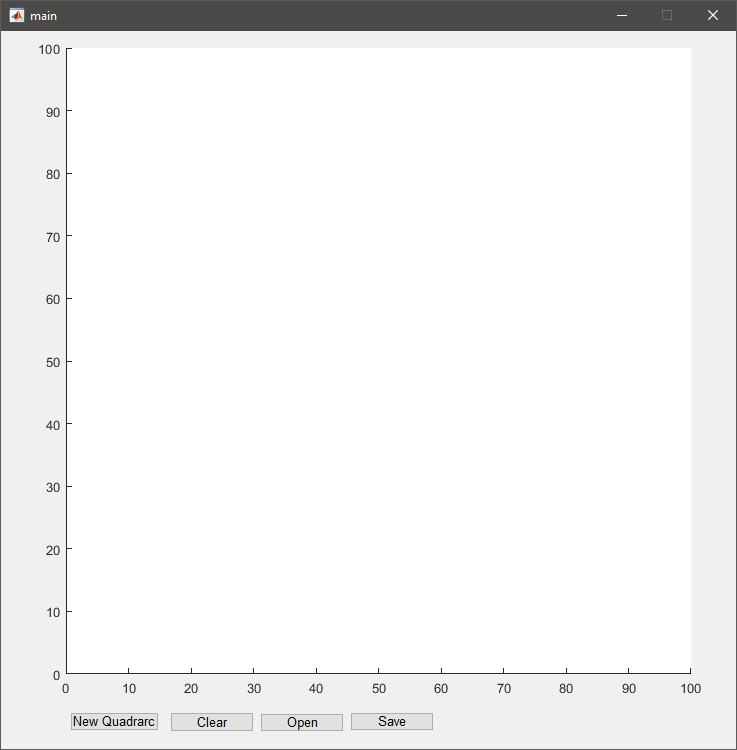
\includegraphics[width=0.25\textwidth]{empty}
%     \caption{A blank plot}
%     \label{fig:empty}
% \end{figure}

% To begin plotting a quadrarc, the user can press the ``New Quadrarc" button. This then changes the cursor to a cross, indicating that the user can draw on the axis. The user can then click and drag on the axis to draw a rectangle. When they release the mouse, they are then presented with an input dialogue which allows them to choose the orientation of the quadrarc, as can be seen in Figure \ref{fig:angle}.

% \begin{figure}[h]
%     \centering
%     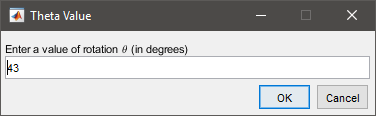
\includegraphics[width=0.25\textwidth]{angle}
%     \caption{Angle choice dialogue}
%     \label{fig:angle}
% \end{figure}

% When the user provides the angle, the rectangle is rotated by that angle. Then the two smaller circles and the two larger circles are plotted in correct orientation with the rectangle. The intersections of the circles are then calculated, and the arcs are then plotted between them to give the ellipse. The final figure can be seen in Figure \ref{fig:done}

% \begin{figure}[h]
%     \centering
%     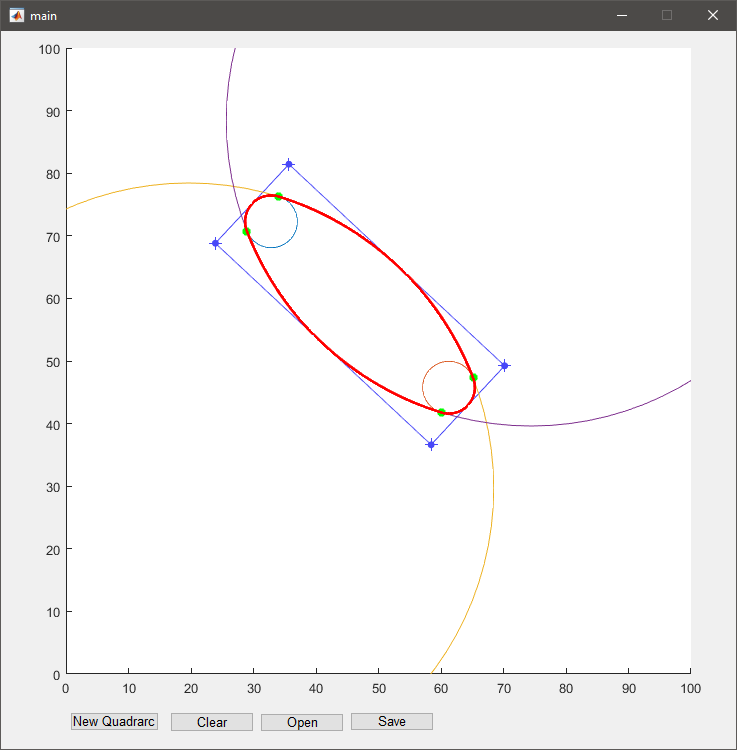
\includegraphics[width=0.25\textwidth]{done}
%     \caption{A plotted quadrarc and construction lines}
%     \label{fig:done}
% \end{figure}

% \subsection{Saving and Loading}

% As well as being able to plot quadrarcs, the user is also able to save and then load plots of quadrarcs. To save a diagram, the user first plots the required quadrarcs. They can then press the ``Save" button and are presented with the system save dialogue. Once the user chooses a location, the diagram is then saved to that location.

% To load a diagram, the user can press the ``Open" button. This opens a file selection dialogue that the user can then select the required \texttt{.fig} file from. Once selected, the current figure is closed and the new one is opened.

% \section{Implementation}
% \subsection{User input}
% For the user interface, I designed the layout using GUIDE. This was as simple as dragging and dropping elements on to the page and then editing metadata about each element.

% To get the location of the rectangle, I used \texttt{getrect()}. This function allows the user to click and drag on an axis and returns the $x$, $y$, width, and height of the rectangle they just drew. Despite there being newer functions available for doing this, I used this one as it returns information useful for calculating the positions and radii of the circles, and not just the coordinates of the vertices.

% To get the angle from the user, I used \texttt{inputdlg()} as it is guaranteed the user will see it as it displays in the middle of the window.

% Finally, for interacting with the file system, I used \texttt{uiputfile()} and \texttt{uigetfile()} methods as these use the system file dialogue so the user will be familiar with how to navigate the file system. 

% \subsection{Algorithm}
% To calculate the position of the two smaller circles, \cite{rosin1999survey} states that the distance from the middle of the rectangle, $h$, should be calculated. This can be calculated using half the width of the rectangle ($a$), and half the height of the rectangle ($b$). $h$ can then be calculated as follows:
% $$
% h=\frac{(a-b)(a+b+\sqrt{a^2+6ab+b^2})}{a-b+\sqrt{a^2+6ab+b^2}}
% $$
% As well as $h$, the distance of the larger circles from the centre of the rectangle ($k$) can be found using the following equation:
% $$
% k=\frac{(a-b)(a+3b+\sqrt{a^2+6ab+b^2})}{4b}
% $$
% As the circles need to be plotted relative to the rectangle, the centre of the rectangle needs to be found. As the \texttt{getrect()} returns the $x$, $y$, width, and height, the centre can be found with
% $$\bigg(x+\bigg[\frac{\textrm{width}}{2}\bigg],y+\bigg[\frac{\textrm{height}}{2}\bigg]\bigg)$$
% The small circles can then be plotted with centres of $(x_{\textrm{r}} \pm h, y_{\textrm{r}})$ and a radii of $a-h$ where $x_{\textrm{r}}$ and $y_{\textrm{r}}$ are the coordinates for the centre of the rectangle \citep{circle}. The large circles can be plotted with centres of $(x_r,y_r\pm k)$ and radii of $b+k$.

% To calculate the coordinates of the intersections, \cite{rosin1999survey} provides the following formula. This provides one of the intersections and the others can be calculated using reflections in the rectangle:
% $$\Bigg(h\Bigg[\frac{a-h}{\sqrt{k^2+h^2}}+1\Bigg],k\frac{a-h}{\sqrt{k^2+h^2}}\Bigg)$$
% The angles between the intersections and the centres of the circles then need to be calculated so that the arcs can be plotted. I used the \texttt{atan2} function to do this. This gives the angle between the horizontal of one point and another. Therefore, to get the angle between the two points, the following formula can be used:
% $$
% \theta = \frac{\pi}{2} - \textrm{atan2}(\delta y,\delta x)
% $$
% Once the two angles for each circles have been found, an arc with the same radius as each circle can be plotted between the two angles of each circle.

% Finally, once all of the points for the circles, rectangle, and arcs have been calculated, they need to be rotated by the angle specified by the user, $\theta$. To do this I used the following rotation matrix:
% \[
% R=
%   \begin{bmatrix}
%     \cos{\theta} & - \sin{\theta} \\
%     \sin{\theta} & \cos{\theta}
%   \end{bmatrix}
% \]
% The issue with the rotation matrix is that it rotates around $(0,0)$. Therefore, for each rotation, I translated the vertices, relative to $(x_r,y_r)$, to $(0,0)$. I then applied the rotation matrix to the matrix of vertices for each shape, and then translated back to the original position.

% \subsection{Clearing the Axis}
% To clear the axis, I used the \texttt{cla()} function provided by MATLAB. I passed the handle to the axis (\texttt{handles.axes1}) to the function, which then cleared the axis.
% \subsection{Loading and Saving}

% To save the figure, I used the built in function \texttt{savefig}. This simply saves the whole figure to a .fig file. This is a binary file that stores the figure object. To load the figure, the \texttt{openfig} function was used. This opens the figure stored in the specified .fig file. As this opens a new figure, I closed the old figure using \texttt{close(handles.figure1)} before opening the new figure.

% % \begin{minted}
% % {matlab}
% % function h = arcGenerator(x,y,r,start, stop)
% % hold on
% % th = start:pi/50:stop;
% % xunit = r * cosd(th) + x;
% % yunit = r * sind(th) + y;
% % h = rot90(cat(1, xunit, yunit));
% % hold off
% % \end{minted}

\bibliographystyle{cardiff}
\bibliography{references}
		
\end{document}